\subsection{Alternatives}

\begin{frame}{Ausgewählte Alternativen zu \alert{The Things Network}}
    \begin{columns}[onlytextwidth]
        \begin{column}{0.15\textwidth}
            
\includegraphics[width=2cm]{material/helium_logo.png}
        \end{column}
        \begin{column}{0.85\textwidth}
        \begin{itemize}
\item Dezentrales Funknetzwerk für IoT‑Geräte.
\item Nutzt Blockchain, um Netzabdeckung zu incentivieren.
        \end{itemize}
        \end{column}
    \end{columns}

    \vspace{0.5cm}

    \begin{columns}[onlytextwidth]
        \begin{column}{0.15\textwidth}
            
\includegraphics[width=2cm]{material/loriot_logo.png}
        \end{column}
        \begin{column}{0.85\textwidth}
        \begin{itemize}
\item Globaler LoRaWAN‑Netzwerkprovider für professionelle Anwendungen.
\item Bietet Optionen für private und öffentliche Netzwerk-Deployments.
        \end{itemize}
        \end{column}
    \end{columns}

    \vspace{0.5cm}

    \begin{columns}[onlytextwidth]
        \begin{column}{0.15\textwidth}
            
\includegraphics[width=2cm]{material/actility_logo.png}
        \end{column}
        \begin{column}{0.85\textwidth}
        \begin{itemize}
\item Fokussiert auf LoRaWAN-Deployments im großen Maßstab.
\item Bietet Netzwerkmanagement, IoT‑Application‑Enablement und mehr.
        \end{itemize}
        \end{column}
    \end{columns}

    \vspace{0.5cm}

    \begin{columns}[onlytextwidth]
        \begin{column}{0.15\textwidth}
            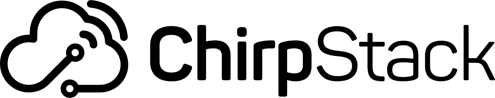
\includegraphics[width=2cm]{material/chirpstack_logo.png}
        \end{column}
        \begin{column}{0.85\textwidth}
        \begin{itemize}
\item Open-Source LoRaWAN Network-Server-Stack.
\item Bietet Flexibilität für das Deployment privater LoRaWAN‑Netze.
\item Geeignet für Enterprise- und industrielle IoT-Anwendungen.
        \end{itemize}
        \end{column}
    \end{columns}
\end{frame}
